\documentclass[12pt]{report}
\usepackage[a4paper,width=150mm,top=25mm,bottom=25mm,bindingoffset=6mm]{geometry}
\usepackage{subcaption} %multiple fig
\usepackage[utf8]{inputenc}
\usepackage{graphicx}
\usepackage{parskip} %package for chaning to new paragraph
\usepackage{sectsty} %for font
\usepackage{amsmath}
\usepackage{caption}
\usepackage{makecell}
\usepackage{apacite}
%\usepackage{pgfplotstable}
\usepackage{inputenc}
\newcommand{\angstrom}{\textup{\AA}}
\numberwithin{equation}{section}

\chapterfont{\centering \LARGE}

\graphicspath{}
\renewcommand{\baselinestretch}{2.0}

\begin{document}

\begin{titlepage} % TITLE PAGE
    \renewcommand{\baselinestretch}{1.5}
    \begin{center}
        \vspace*{0.5cm}
 
        \large
        \textbf{TOWARDS PREDICTION OF OPTIMAL ALCOHOL ANTIFREEZE STRUCTURAL 
        FEATURES USING THE EXTREME GRADIENT BOOSTING METHOD WITH OPTIMIZATION}
 
        %\vspace{0.25cm}
        %\LARGE
        %Thesis Subtitle
 
        \vspace{0.5cm}
        \Large
        \textbf{Phong Ho}
 
        \vspace{0.5cm}

        \Large
 
        a Thesis Presented for the Degree of\\
        Bachelor of Engineering
 
        %\vspace{0.8cm}
        \vfill
 
        
\includegraphics[width=0.4\textwidth]{qlogo.png}
        \vfill
 
        \large
        Department Name: Mechanical Engineering\\
        Research Supervisors:\\
        Prof. Hiroshi Takamatsu\\
        Assoc. Prof. James Cannon\\
        August, 2019
 
    \end{center}
\end{titlepage} %Title page
\newpage
\addcontentsline{toc}{chapter}{Acknowledgement}
\chapter*{Acknowledgements}
\thispagestyle{plain}
I am thankful for being a member of this project, for
the people that I have been with and cooperate and 
for the experience i have gained professionally and individually that support my self development
\\
I owe my appreciation to Prof. James J Cannon for being an understanding advisor, 
a friend and an important teacher. I am thankful to him for providing me a 
freedom of research environment, a chance to explore myself professionally and 
personally, for providing me personal advices when I was in crises and for 
letting me try my most non-sense ideas.\\
I send my gratitude to Prof. Hiroshi Takamatsu for accepting me into this 
laboratory, for being personally and professionally supportive by 
constructive critisms and advices that I would never think of without him,
for sharing me his favourite drink and for showing me the world of research.\\
I am grateful to Prof. Kurata and all of former and current Heat and Mass Transfer
laboratory members that I have met, for being so kind, for helping me blend in 
the culture difference, for all of the professional advices and for giving me 
unforgettable memories.\\
I greatly appreciate my best friend Tuan Do for all of his support in my 
personal and professional life. Without his lessons, I could not have been 
able to finish this work. Without his mid-night talks, I could have quit 
mid-way because of depression and lost of direction.\\
I am also lucky to have wonderful friends in my IUPE (G30) program for always 
supporting me through my hard times and for being a part of my memorable 
university life.\\
Finally, I owe my greatest appreciation to my family, my father, my mother,
my sister and my cousin for being the 
strongest mental support and for trusting me, giving me a chance to be who 
i am today. %Acknowledgement
\newpage
\tableofcontents
\addcontentsline{toc}{chapter}{List of Figures}
\listoffigures

\newpage
\chapter*{Abstract}
\thispagestyle{plain}
\begin{center}
    \renewcommand{\baselinestretch}{1.5}
    \Large
    \textbf{TOWARDS PREDICTION OF OPTIMAL ALCOHOL ANTIFREEZE STRUCTURAL 
    FEATURES USING THE EXTREME GRADIENT BOOSTING METHOD WITH OPTIMIZATION}
 
    %\vspace{0.4cm}
    %\large
    %Thesis Subtitle
 
    \vspace{0.4cm}
    \large
    \textbf{Phong Ho}
 
    %\vspace{0.9cm}
    %\textbf{Abstract}
\end{center}

In this research, we used a statistical approach to find a research direction 
as well as to predict structural features of the next generation of alcohol 
coolant, studying from 8 types of alcohol: methanol, ethanol, ethylene glycol, 
1-propanol, 2-propanol, glycerol, 1,3-propanol and propylene glycol. 
The statistical approach is done by implementing a supervised machine 
learning technique named extreme gradient boosting while the experimental 
data for the statistical technique is obtained from the Green-Kubo relation 
based molecular dynamics simulations.

The results showed that the machine learning models can predict values from 
what they have learned. However, the models could not perform well for the 
data that has a different pattern than the training data. The results also 
suggest that to solve this problem, these 2 solutions should be taken in 
action: diversify the training data and conduct research on special alcohol 
types.\\
The machine learning approach can also show the influence of structural 
features on thermal conductivity and viscosity, which from that further 
research can be conducted to examine the underlying mechanism of those 
features.\\
The optimization part successfully predicted the structural features of 
the next potential candidate from the given alcohol sample. However, a 
future improvement of variable set and an interpreting method need to be 
developed in order to construct a complete molecular structure. %Abstract

\chapter{Introduction} %Introduction
\section{Research Background}
Choice of a cooling system is inevitable in many applications since the 
involvement of heat transfer is important in many industries such as 
automobiles, architecture and electronics. The cooling system plays 
an important role in managing the system temperature, preventing the 
operating system from being overheated, which could lead to severe 
consequences if it is not taken seriously. Compared to the development 
of cooling technologies, the development of the cooling medium itself is 
often less considered. The choosing of an appropriate coolant would improve 
the performance as well as reduce cost for building the system.

Among liquid coolants, water is considered to be one of the best 
candidates for coolants with its high heat capacity and low viscosity 
\cite{mohapatra_advances_2005}. However, the temperature range of 
water in the form of liquid is only from $0^\circ$C to $100^\circ$C, 
which is a relatively small range. If the system 
temperature gets out of the range, the expansion of ice or the evaporation 
of vapor could cause unexpected behaviors, which can lead to the break down 
of the entire system. 

One of the ideas to overcome this problem is to create an aqueous-based 
solution with an alcohol to expand the operational temperature range while 
keeping the good performance in heat transfer and low viscosity. Many alcohol 
types have been introduced for this approach, such as propylene glycol, 
ethylene glycol, methanol or ethanol. However, their low thermal conductivity 
as well as high viscosity become a burden for the cooling medium. Thus, the 
finding of new alcohol in cooling is necessary. However, while there are an 
enormous number of possibilities, the cost of conducting an experiment is not 
neglectable, not to mention that we do not have a clear direction to research 
towards the goal.

Such problems can be overcome if we can create functions that link 
molecular structure features to the values of desired properties such as 
thermal conductivity and viscosity. With such a function, we can adjust any 
structural feature to obtain corresponding property values as well as study 
further on existing database, we can be correctly oriented to reach the 
optimal coolant that satisfy all the desired property constraints.

Such functions can be obtained with the help of computational power such 
as molecular dynamics simulations and supervised machine learning. 
In this work, we develop a methodology that help us get a research 
direction as well as predict the molecular structural features of 
next-generation alcohol coolants for future antifreeze development 
using molecular simulation code LAMMPS for computer simulations combined 
with supervised machine learning using the eXtreme Gradient Boosting technique.
\section{Why use computational methods?}
To understand why computational power is such a perfect vehicle to deliver 
the answer for this problem, we will introduce the two computational 
techniques and how can they bring great benefits for this type of problem.
\subsection{Supervised machine learning method}
Supervised machine learning is a class of advanced computing and statistical 
techniques that maps a function of given sets of input-output. In other words, 
if the input is information of structural features and the output is desired 
properties, we can obtain the function that we desired as mentioned earlier. 
This is a highlight of implementing the computational method since conducting 
the function by analytical method would take a great amount of time and effort, 
not to mention the difficulty. However, using supervised machine learning 
requires a large amount of data in order to obtain accurate and acceptable 
results. Thus, the perfect combination for machine learning is molecular 
dynamics simulations.
\subsection{Molecular Dynamics simulation}
Molecular dynamics simulation is a computational system that numericalizes 
features and behaviors of atoms and molecules. We will discuss the details 
of molecular dynamics in the next section while here I will give some details 
of notable advantages of molecular dynamics in relation to this problem. 
Compared to manual experimental methods, molecular dynamics simulations 
brings much greater benefits.\\
Molecular dynamics simulations require information of the environment, 
such as system volume, temperature, pressure and numerical information 
of investigated coolants, and appropriate computational power to conduct 
an experiment and calculate thermophysical properties. In that sense, 
it is much safer and precise in terms of environment control as well as 
simpler in terms of experimental setup, which saves a lot of resources.\\
By being able to control the process to every single detail, we also can have 
a more insight of atomic behaviors inside the system, in spite of the 
difficulty of observing it if we conduct the experiment traditionally.\\
Standing out from the above benefit, simulations can significantly reduce the 
time to conduct experiments. The entire process is automated with the human 
factor as an observer which allows the experiments to run continuously, 
avoiding the gap that exists in traditional experiments due to human body 
limitation, yet, without compromising the accuracy. To elevate this ability, 
simulations also can run in parallel, which means we can conduct several 
experiments at the same time; the number depending only on the available 
computational power; and the accuracy is still guaranteed.\\
Thus, we can escalate the number of experiments and get much greater amount 
of data with much shorter time to serve the machine learning purpose.
\newpage\section{Thesis Outline}
The thesis is presented in the following manner:

\textbf{Chapter 1 - Introduction} 
\\Providing the background of the research, the idea 
to tackle the problem that we want to answer as well as the reason why 
we have that idea, an introduction about why computational methods should 
be applied to solve this problem.

\textbf{Chapter 2 - Theory} 
\\Providing information of background knowledge that we need 
to know in order to understand the approach that we are about to propose. 
The background knowledge includes the Green-Kubo formulas of thermal 
conductivity and viscosity, molecular dynamics simulations, and all the 
relevant machine learning related techniques.

\textbf{Chapter 3 - Method} 
\\Providing information of how to operate the approach in 
detail, including cultivating data method and data processing method.

\textbf{Chapter 4 - Results and Discussion} 
\\Providing the results of models 
in different situations, the results from optimization process and discussion 
about the results.

\textbf{Chapter 5 - Conclusion} 
\\Summary the entire work. %Input intro.tex
\newpage
\chapter{Theoretical Background} %Chapter 2 Title - alcohol analytic compare with literature, finding variables
To be able to understand the method, we will introduce a few theoretical 
backgrounds that are related to the tools I will use in this research.
\section{Molecular Dynamics Simulation}
As mentioned in the previous chapter, molecular dynamics simulation is 
a numerical system that describe atomic status over time in a specified 
environment. From the cultivated information, we can either investigate 
the atomic behaviors or calculate thermophysics properties such as thermal 
conductivity and viscosity easily. A standard molecular dynamics simulation 
has an algorithm as follows \cite{manjunatha_development_2018}
\begin{figure}
    \begin{center}
        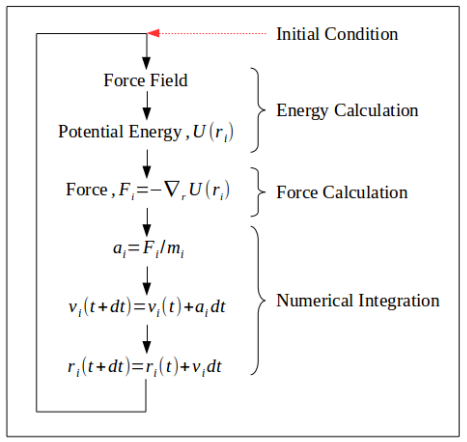
\includegraphics[width=0.75\textwidth]{mdalgo.png}
    \end{center}
    \caption{Basic outline of a MD simulation}
\end{figure}
\newpage
The initial conditions describe the initial state of the atoms such as 
velocity $v(t_0)$, mass of atom $m$ and coordination $r(t_0)$. For atoms of a liquid, given the $i^{th}$ atom, 
the initial coordination $r_i(t_0)$ is randomized along with several 
constraints such as structural constraints (angles, bond lengths) 
and displacement constraints to avoid malfunction in the system as well as 
systematic errors. The initial velocity $v_i(t_0)$ is randomized on the Gaussian 
distribution with the constraint that the total momentum of the entire system 
is $0$.

After the initial setup, a class of functions called a force field is used 
to calculate the potential energy $U_i = U(r_i)$ which is a function of position 
that obeys the structural constraints of the atom. The obtained potential 
energy $U(r_i)$ can be used to deduce the forces $F_i$ that apply on the atom.

The force $F_i$ is then processed by using Verlet algorithm as follows to obtain 
the functions of velocity and position over time. For a time step $\Delta t$, 
the function that presents the position of the $i^{th}$ atom after $\Delta t$ is
\begin{equation}
    r_{i}(t+\Delta t) \approx r_{i}(t)+\Delta t \dot{r}_{i}(t)+\frac{1}{2} \Delta t^{2} \ddot{r}_{i}(t)\label{eq:2.1.1}
\end{equation}
To get the velocity term after a time step $\Delta t$, we have to deduce $r_i(t)$ 
backwards from $r_i(t+\Delta t)$. Thus
\begin{equation}
    r_{i}(t) \approx r_{i}(t+\Delta t)-\Delta t \dot{r}_{i}(t+\Delta t)+\frac{1}{2} \Delta t^{2} \ddot{r}_{i}(t+\Delta t)\label{eq:2.1.2}
\end{equation}
Substituting \ref{eq:2.1.2} into \ref{eq:2.1.1} we get
\begin{equation}
    \dot{r}_{i}(t+\Delta t)=\dot{r}_{i}(t)+\frac{1}{2} \Delta t\left[\ddot{r}_{i}(t)+\ddot{r}_{i}(t+\Delta t)\right]
\end{equation}
Or
\begin{equation}
    \dot{r}_{i}(t+\Delta t)=v_{i}(t+\Delta t)=v_{i}(t)+\frac{1}{2 m_{i}} \Delta t\left[F_{i}(t)+F_{i}(t+\Delta t)\right]
\end{equation}
The values of positions and velocities at $t+\Delta t$ will be served as the next 
initial condition for the next loop of calculation until the set running time 
T is reached. The values of positions and velocities will be used to calculate 
thermal conductivity and viscosity by using a deduction of the Green-Kubo 
relation.
\section{Green-Kubo Relation}
Green-Kubo relation is a formula that shows the relationship between the 
transport coefficient and the dynamical variables. 
The general expression is as follows \cite{hansen_theory_2013}
\begin{equation}
    K=C \int_{0}^{\infty}\langle D(t) D(0)\rangle \mathrm{d} t
\end{equation}
Where K is the transport coefficient, 
D is dynamical variable terms 
and C is the function constant. To be able to calculate viscosity and 
thermal conductivity values, the Green-Kubo expression will be transformed, 
without detailed derivation delivered, and presented as follows
\subsection{Viscosity}
The Green-Kubo expression for calculating viscosity is as follows:
\begin{equation}
    \eta=\frac{V}{k_{b} T} \int_{0}^{\infty}\left\langle P_{\alpha \beta}(t) \cdot P_{\alpha \beta}(0)\right\rangle d t
\end{equation}
Where $P$ is stress tensor terms, 
$\alpha,  \beta \in (x, y, z)$ is the 3D direction, 
V is the system volume, 
T is the system temperature, 
$k_B=1.38 \times 10^{-23}$ $[m^2\cdot kg\cdot s^{-2}\cdot K^{-1}]$ is the Boltzmann constant 
and $\langle \rangle$ is the ensemble average \cite{hansen_theory_2013}.\\
Furthermore, the stress tensor terms can also be expressed as follows:
\begin{equation}
    P_{\alpha \beta}=\frac{1}{V}\left(\sum_{i} m_{i} v_{i_{\alpha}} v_{i_{\beta}}+\sum_{i} r_{i_{\alpha}} f_{i_{\beta}}\right)
\end{equation}
Where $m$ is the atom mass, $v$ is the atom velocity, $r$ is the atom position, 
$f$ is the forces act on atom and $i$ is the atom index \cite{allen_time_2017}.
\subsection{Thermal Conductivity}
The Green-Kubo expression for calculating thermal conductivity is as follows:
\begin{equation}
    \lambda_{T}=\frac{V}{k_{\mathrm{B}} T^{2}} \int_{0}^{\infty} \mathrm{d} t\left\langle J_{\alpha}(t) J_{\alpha}(0)\right\rangle
\end{equation}
Additionally, J is heat flux terms, 
V is the system volume, 
T is the system temperature, 
$k_B=1.38 \times 10^{-23}$ $[m^2\cdot kg\cdot s^{-2}\cdot K^{-1}]$ is the Boltzmann constant, 
$\langle \rangle$ is the ensemble average and
$\alpha \in (x, y, z)$ is the 3D direction \cite{hansen_theory_2013}.\\
Furthermore, The heat flux terms can be broken down further. Thus,
\begin{equation}
    J_{\alpha}=\frac{1}{V}\left(\sum_{i} e_{i} v_{i}+\sum_{i<j}\left(f_{i j} \cdot v_{j}\right) r_{i j_{\alpha}}\right)
\end{equation}
Where $e$ is energy per-atom, 
$v$ is the velocity of atoms, 
$f$ is the force between atoms, 
$r$ is the distance between atoms in the $\alpha$ direction and 
$i$ and $j$ are the atom indices \cite{manjunatha_development_2018}.
\section{eXtreme Gradient Boosting Method}
eXtreme Gradient Boosting (XGBoost) method is a robust supervised machine 
learning method that consists of different advanced statistical techniques. 
The advanced statistical techniques help XGBoost achieve a high calculation 
speed and accuracy. To be able to understand XGBoost for the purpose of this 
research, the following XGBoost component techniques will be explained\\
- Gradient boosting\\
- Regularization object\\
- Sub-sample \& sub-column
\subsection{Gradient Boosting}
The gradient boosting feature improves the accuracy of model prediction 
ability and calculation speed. Gradient boosting consists of 2 parts: 
boosting and gradient.
\subsubsection*{Boosting}
From a mathematical perspective, the boosting algorithm is similar to the 
Lagrange Multiplier method. Given a sample data set of n elements to make 
the XGBoost model, the mission of boosting is to minimize the loss function
$\sum_{i=1}^{n} l\left(y_{i}, \hat{y_{i}}\right)$, 
which is the total sum of differences between predicted values and actual 
values, so that the predicted outcomes are closest to the actual values. 
The boosting algorithm also involves creation of multiple sub-functions from 
given variables which serve as constraints for the Lagrange problem. Finally, 
boosting algorithm takes an adjustable coefficient as the Lagrange Multiplier 
coefficients. Instead of having many coefficients as is typically used in the 
Lagrange multiplier method, boosting only uses a unified coefficient to avoid 
unnecessary complexity for the system while it does not have to compromise too 
much on accuracy. The boosting algorithm can be represented by the following 
expression, where $\hat{f}_b(x)$ represents each sub-function that boosting creates and 
$\lambda$ represents the Lagrange coefficient:
\begin{equation}
    0 \leftarrow \sum_{b=1}^{B} \sum_{i=1}^{n} l\left(r_{i}, \hat{r}_{i}\right)_{b}+\sum_{b=1}^{B} \lambda \hat{f}_{b}(x)
\end{equation}
Which can be written as:
\begin{equation}
    0\leftarrow \sum_{i=1}^{n} l\left(y_{i}, \hat{y}_{i}\right)+\sum_{b=1}^{B} \lambda \hat{f}_{b}(x)
\end{equation}
Furthermore, B is the total number of sub-functions, n is the number of data 
in the sample data and r is the difference between actual values and predicted 
values of the previous sub-function. For example, for any data point i in the 
data sample being processed by sub-function b:
$r_{i}^{b}=y_i^{(b-1)}-\hat{y}_i^{(b-1)}$. 
Initially, $r_{i}^{0}=y_i$ \cite{james_introduction_2013}.
\subsubsection*{Gradient}
Instead of $\sum_{i=1}^{n} l\left(y_{i}, \hat{y_{i}}\right)$, the loss function
is expanded by the Taylor expansion to the second degree, which is where the terms 
“gradient” comes from. Thus, at any $t^{th}$ sub-function, the loss function becomes:
\begin{equation}
    \sum_{i}^{n_{t}}\left[l\left(r_{i}, \hat{r}_{i}^{(t-1)}+\hat{f}_t\left(x_{i}\right)\right)]\right.
\end{equation}
\begin{equation}
    \sum_{i=1}^{n_t}\left[l\left(r_{i}, \hat{r}^{(t-1)}\right)+g_{i} \hat{f}_t\left(\mathbf{x}_{i}\right)+\frac{1}{2} h_{i} {\hat{f}_{t}^{2}}\left(\mathbf{x}_{i}\right)\right]
\end{equation}
Where $g_{i}=\partial_{\hat{r}^{(t-1)}} l\left(r_{i}, \hat{r}^{(t-1)}\right)$ and
$h_i=\partial_{\hat{r}^{(t-1)}}^{2} l\left(r_{i}, \hat{r}^{(t-1)}\right)$ are 
the Taylor expansion coefficients. By expanding into 2nd degree of Taylor expansion, 
the loss function will converge faster and more accurately while avoiding 
overfitting \cite{chen_xgboost:_2016}.\\
Overfitting refers to the performance of a model that is particularly good for a specific set 
of data and consequently may not be able to produce reliable predictions. 
\subsection{Regularization Object}
Regularization is a technique that identifies unnecessary or less important 
variables by shrinking the coefficient of all variables (the coefficients 
inside the sub-functions, which are different from the Lagrange coefficient) 
towards zero. The coefficients of unnecessary or less important variables will 
become zero, thus, do not affect the model \cite{james_introduction_2013}. To control 
the regularization process, the XGBoost method has 2 parameters, the LASSO 
parameter \cite{tibshirani_regression_1996} and the Ridge Regression parameter \cite{hoerl_ridge_1970}.
\subsection{Subsample \& Subcolumn}
Machine learning techniques normally use a set of sample data (training data) 
to create the component functions. However, using the entire training data set 
often encounters overfitting problems. Thus, XGBoost introduces sub-sample and sub-column features.

Sub-sample is a technique that instead of using the entire training data set, 
the algorithm only uses a portion of it.
Sub-column is similar to sub-sample but instead of using a part of training data, 
the algorithm uses a subset of the available variables.
Thus, for each sub-function, a different set of sub-sample and sub-column will 
be implemented. By doing so, the algorithm can prevent overfitting and detect 
the relationship between variables and outcomes even further and use of 
sub-columns also increase the computing speed \cite{chen_xgboost:_2016}.

Corresponding to the explained theory, XGBoost has the following parameters 
that need to be chosen:\\
- n\_estimators = number of sub-functions B\\
- learning\_rate = the Lagrange coefficient $\lambda$\\
- subsample = sub-sample size\\
- colsample\_bytree = sub-column size\\
- reg\_alpha = the LASSO parameter\\
- reg\_lambda = the Ridge Regression parameter


\section{Cross Validation}
Every predictive model for a purpose comes along with a prediction error 
(true error), which show how different the outputs of the model compared 
to the true values of the corresponding inputs. Cross validation is a method 
that estimates the true error of a predictive model. For sample data, which 
includes both input and true values of output, the estimation of error is a 
simple job. However, for real data, the true error is usually unable to be 
found due to the absence of the true values of output. Thus, cross validation 
is implemented to approximate the true error from existing data sets 
\cite{rodriguez_sensitivity_2010}.
\subsection*{k-folds method}
The k-folds method is a cross validation method that’s popularly used in 
machine learning because of its good performance. In the k-fold method, 
the sample data set of n data points is divided into k equal $\frac{n}{k}$ data point 
portions with no shared component. The ith portion will be used to test the 
model (validation set) and give a numerical test error while the other k-1 
portions will be used to train the model (training set). The process iterates 
k times so that every portion would be selected as test set once. The true 
error of the model will be estimated by averaging k numerical values of test 
error. The error measuring error for numerical output problem can be mean 
square error method as follows:
\begin{equation}
    M S E=(y-\hat{y})^{2}
\end{equation}
Where $y$ is the real value and $\hat{y}$ is the predicted value. Thus, the 
true error estimation becomes
\begin{equation}
    True Error Estimation=\frac{1}{k} \sum_{i=1}^{k} \sum_{j=1}^{n_i}\left(y_{j}-\hat{y}_{j}\right)_{i}^{2}
\end{equation}
Where i is the index of divided portions, j is the index of data points and 
$n_i$ is the data in the $i^{th}$ portion. The k-folds method helps us to 
reduce the variance of models’ training scores, which due to the splitting of 
validation set and training set, and estimate the most stable performance scores. %Input chap2.tex
\chapter{Method} %Chapter 3 Title - method, writing specifically about Green Kubo formulation, then say lammps, xgb, opt
In this work, we will investigate alcohol-water mixtures of 8 different 
alcohols with the solution concentrations varying from 2\% to 50\% for each.
The investigated alcohols include:\\
- ethylene glycol\\
- ethanol\\
- methanol\\
- glycerol\\ 
- 1-propanol\\
- 2-propanol\\ 
- 1,3-propanediol\\
- propylene glycol\\
as they are alcohol types that were used as industrial antifreeze.
The methodology is operated according to the following diagram
\begin{figure}
    \begin{center}
        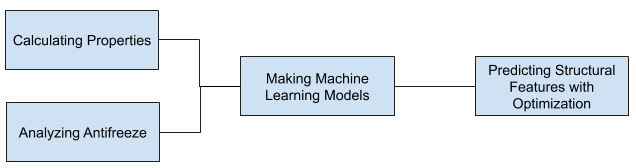
\includegraphics[width=1\textwidth]{method.png}
    \end{center}
    \caption{Procedure of the Methodology}
\end{figure}
\section{Calculating Properties}
In this work, the calculations of properties are carried out by LAMMPS \cite{plimpton_fast_1995}.
Since the investigated objects are water-alcohol mixtures, the fundamental inputs include\\
- Number of alcohol molecules\\
- Number of water molecules\\
- Declaring implemented alcohol molecular model\\
- System temperature T\\
- System volume V\\
- System pressure P\\
TIP4P/Ice \cite{abascal_potential_2005} will be used as the water model throughout all 
mixtures while all alcohol models are based on OPLS-AA \cite{jorgensen_development_1996}, 
which is derived from the Optimized Potentials for Liquid Simulations models 
\cite{jorgensen_opls_1988}.The system pressure is set at 1 atm while the volume of the 
system is set at 40x40x40 $\textup{\AA}^3$ throughout all simulations.\\
Since we are investigating throughout the mass concentration of mixtures, 
we construct a small converter that approximate the number of alcohol 
molecules and water molecules from input mass concentrations. Assuming 
that the sum of volume of water and volume of alcohol equals the system 
volume, we obtain the following:
\begin{equation}
    m_{w}=\rho_{w} V_{w}
\end{equation}
\begin{equation}
    m_{w}=\rho_{w}\left(V-V_{a l c}\right)
\end{equation}
\begin{equation}
    m_{w}=\rho_{w}\left(V-m_{a l c} / \rho_{a l c}\right) \label{eq:1}
\end{equation}
Where $m_w$ is mass of water, $\rho_w$ is density of water, $V_w$ is volume 
of water, $m_{alc}$ is mass of alcohol, $\rho_{alc}$ is density of alcohol and
$V_{alc}$ is volume of alcohol.\\
But then the mass concentration is:
\begin{equation}
    c_{\%}=\frac{m_{alc}}{m_{a k}+m_{alc}}
\end{equation}
Thus
\begin{equation}
    m_{alc}=\frac{c_{\%}}{1-c_{\%}}m_w  \label{eq:2}
\end{equation}
Substitute \ref{eq:2} into \ref{eq:1} we obtain
\begin{equation}
    m_{w}=\rho_{w}\left(V-\frac{c_{\%}}{1-c_{\%}} m_{w} / \rho_{a l c}\right)
\end{equation}
Collect all the terms that contain $m_w$ into one side then eliminate the coefficients, we obtain:
\begin{equation}
    m_{w}=V \rho_{a l c} \rho_{w}\left(1-c_{\%}\right) /\left(\rho_{w} c_{\%}+\left(1-c_{\%}\right) \rho_{a l c}\right)
\end{equation}
\begin{equation}
    m_{a l c}=\frac{1-c_{\%}}{c_{\%}} m_{w}
\end{equation}
Thus, the number of alcohol molecules $N_{alc}$ and the number of water molecules $N_w$
can be obtained as follows:
\begin{equation}
    N_{a l c}=N_{A} \frac{m_{a l c}}{M_{a l c}}
\end{equation}
\begin{equation}
    N_{w}=N_{A} \frac{m_{w}}{M_{w}}
\end{equation}
Furthermore, $N_A$ is the Avogadro number, $M_{alc}$ is the molar mass of alcohol and 
$M_w$ is the molar mass of water.

The method is validated by taking the calculated number of molecules to 
calculate the mass concentration. The error between calculated mass 
concentrations and input concentrations do not surpass 2\%. Thus, the method 
is valid. The error arises from the fact that an integer number of molecules 
is required.\\
The densities of pure liquid are taken from online chemistry database CHERIC 
(Chemical Engineering and Materials Research Information Center) under 
conditions of 1 atm and 293K. Thus, the temperature of systems are set at 
293K and 1 atm pressure.\\
The thermal conductivity can be deconstructed into 2 terms: virial and 
convective. The virial terms represents the interatomic interaction 
contribution to the thermal conductivity while the convective terms show the 
diffusion in the thermal conductivity. It is shown that the virial terms 
dominate the convective terms and can be used to represent the trend of 
values \cite{lin_constructing_2011}. Furthermore, in LAMMPS, the calculation time of 
the virial terms is much shorter compared to the total thermal conductivity 
due to the absence of the enthalpy quantity that is required to calculate the 
total term. Since the main aim of this work is the trend of values instead of 
the absolute values themselves, to reduce calculation costs, only the virial 
term is calculated. However, we can still calculate the total terms for 
viscosity since we do not need enthalpy quantity for viscosity calculations.


\section{Analyzing Antifreeze Molecules}
Since the purpose is to make a function of structural features to desired 
properties, in this section, we will discuss about which features should be 
chosen as variables for the functions. The variables’ roles are not only to 
form relationships to desired properties, but also to distinguish different 
data points. To avoid unnecessary complexity, the variables (or structural 
features) should be independent.

In alcohol, it is already understood that the number of OH groups 
significantly affect the ability of heat transfer while the position of the OH 
group also change the properties values \cite{manjunatha_investigation_2017}. However, there 
might be also other potential structural features that are left uninvestigated. 
Since we only care about the impact of the structural features on the 
thermophysical properties, we will select all the features that define an 
alcohol molecular structure.
\newpage
\begin{figure}[h!]
    \centering
    \begin{subfigure}[b]{0.3\linewidth}
      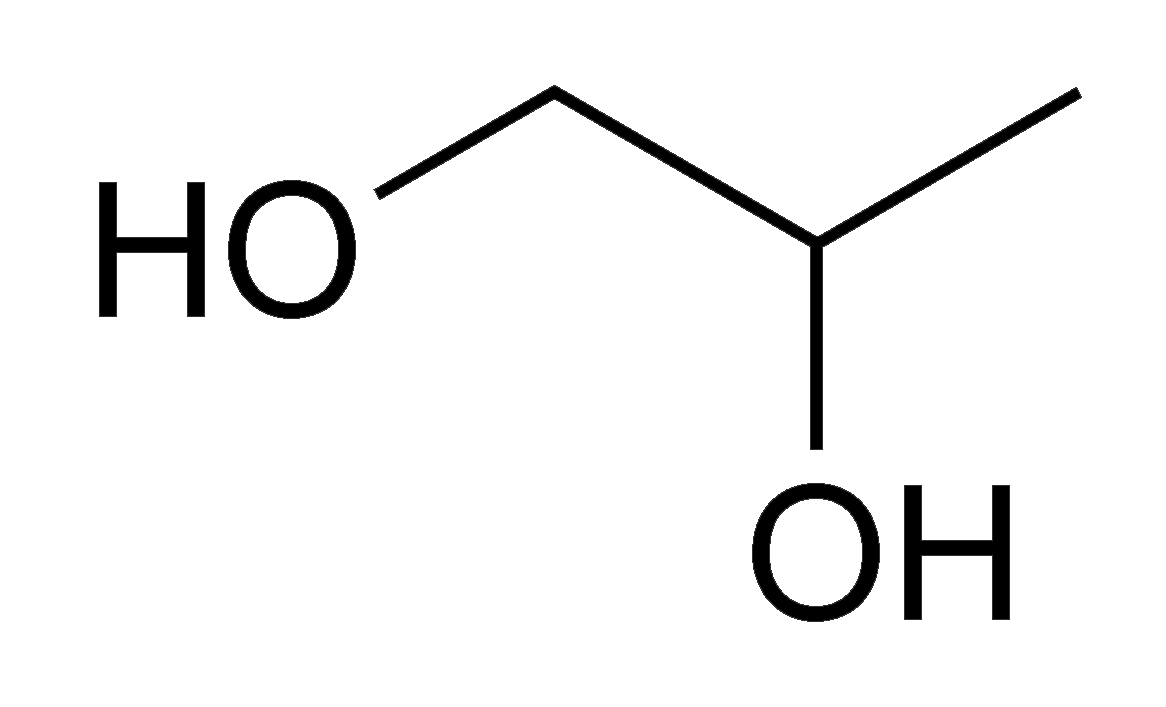
\includegraphics[width=\linewidth]{prplene.png}
       \caption{Propylene Glycol}
    \end{subfigure}
    \begin{subfigure}[b]{0.3\linewidth}
      
\includegraphics[width=\linewidth]{13prop.png}
      \caption{1,3-propanediol}
    \end{subfigure}
    \begin{subfigure}[b]{0.3\linewidth}
        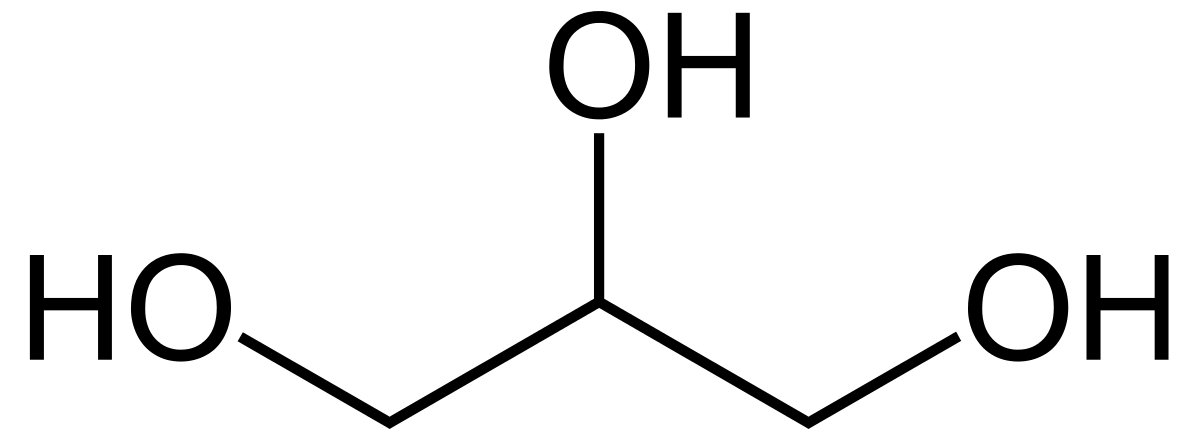
\includegraphics[width=\linewidth]{glycerol.png}
        \caption{Glycerol}
      \end{subfigure}
    \begin{subfigure}[b]{0.3\linewidth}
      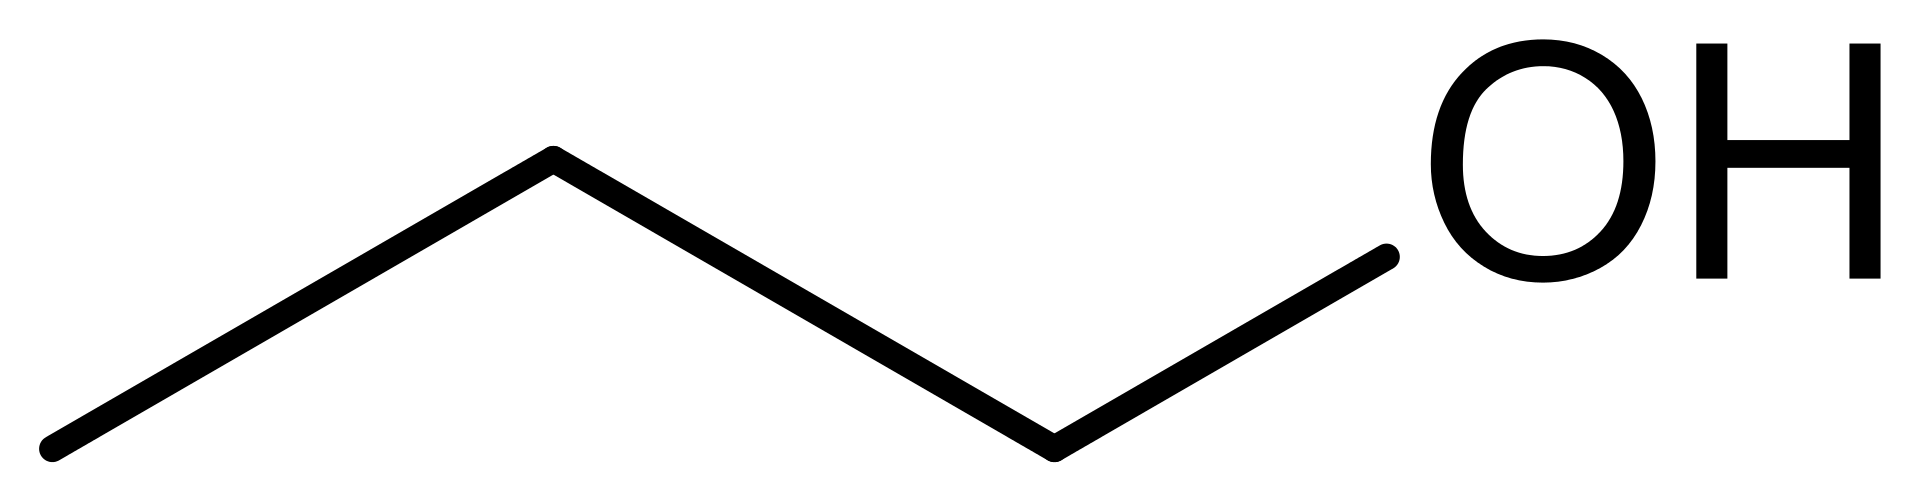
\includegraphics[width=\linewidth]{1prop.png}
      \caption{1-propanol}
    \end{subfigure}
    \begin{subfigure}[b]{0.3\linewidth}
      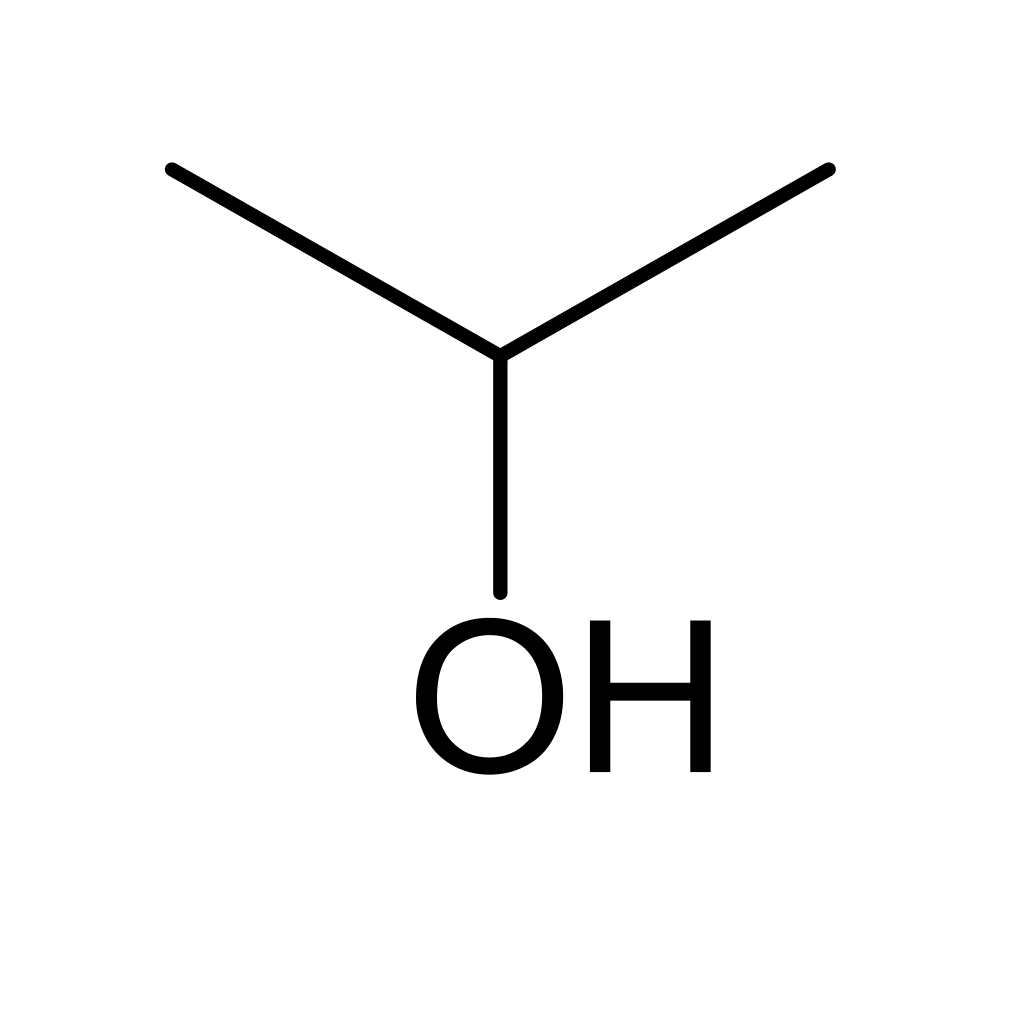
\includegraphics[width=\linewidth]{2prop.png}
      \caption{2-propanol}
    \end{subfigure}
    \begin{subfigure}[b]{0.3\linewidth}
        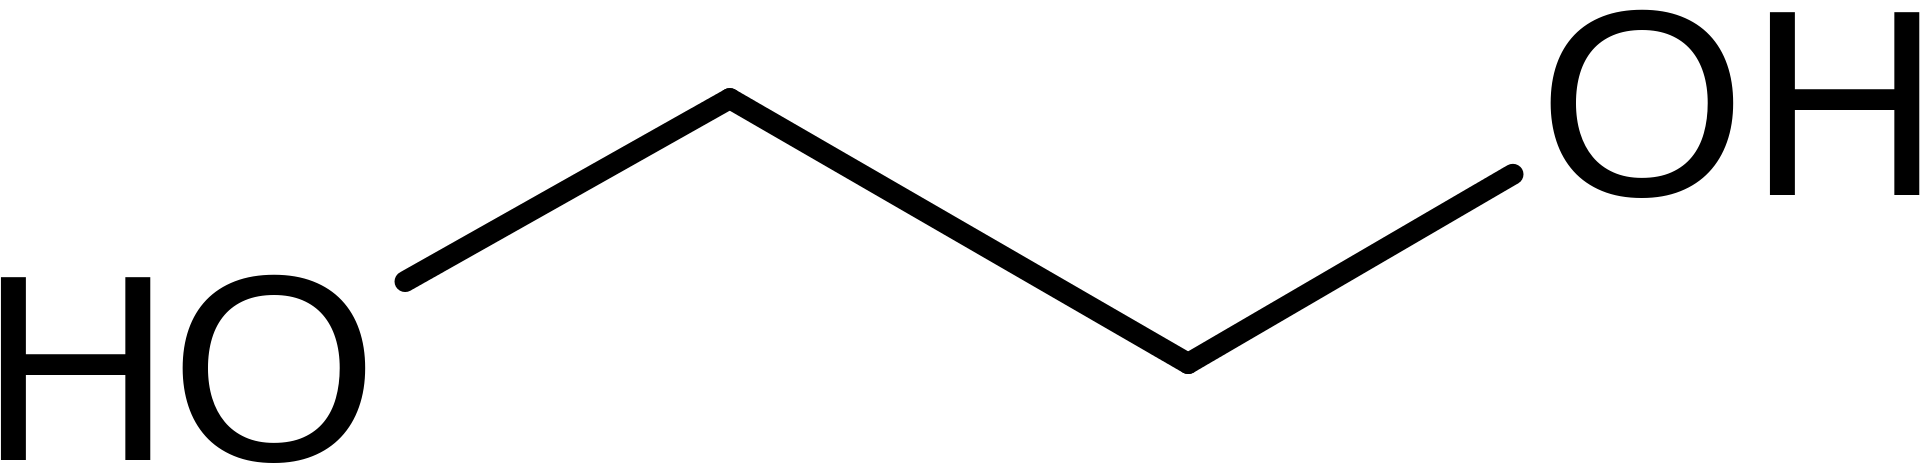
\includegraphics[width=\linewidth]{ethlne.png}
        \caption{Ethylene Glycol}
      \end{subfigure}
      \begin{subfigure}[b]{0.3\linewidth}
        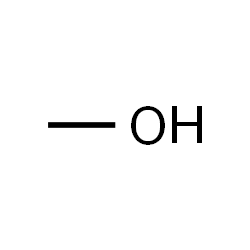
\includegraphics[width=\linewidth]{meth.png}
        \caption{Methanol}
      \end{subfigure}
      \begin{subfigure}[b]{0.3\linewidth}
        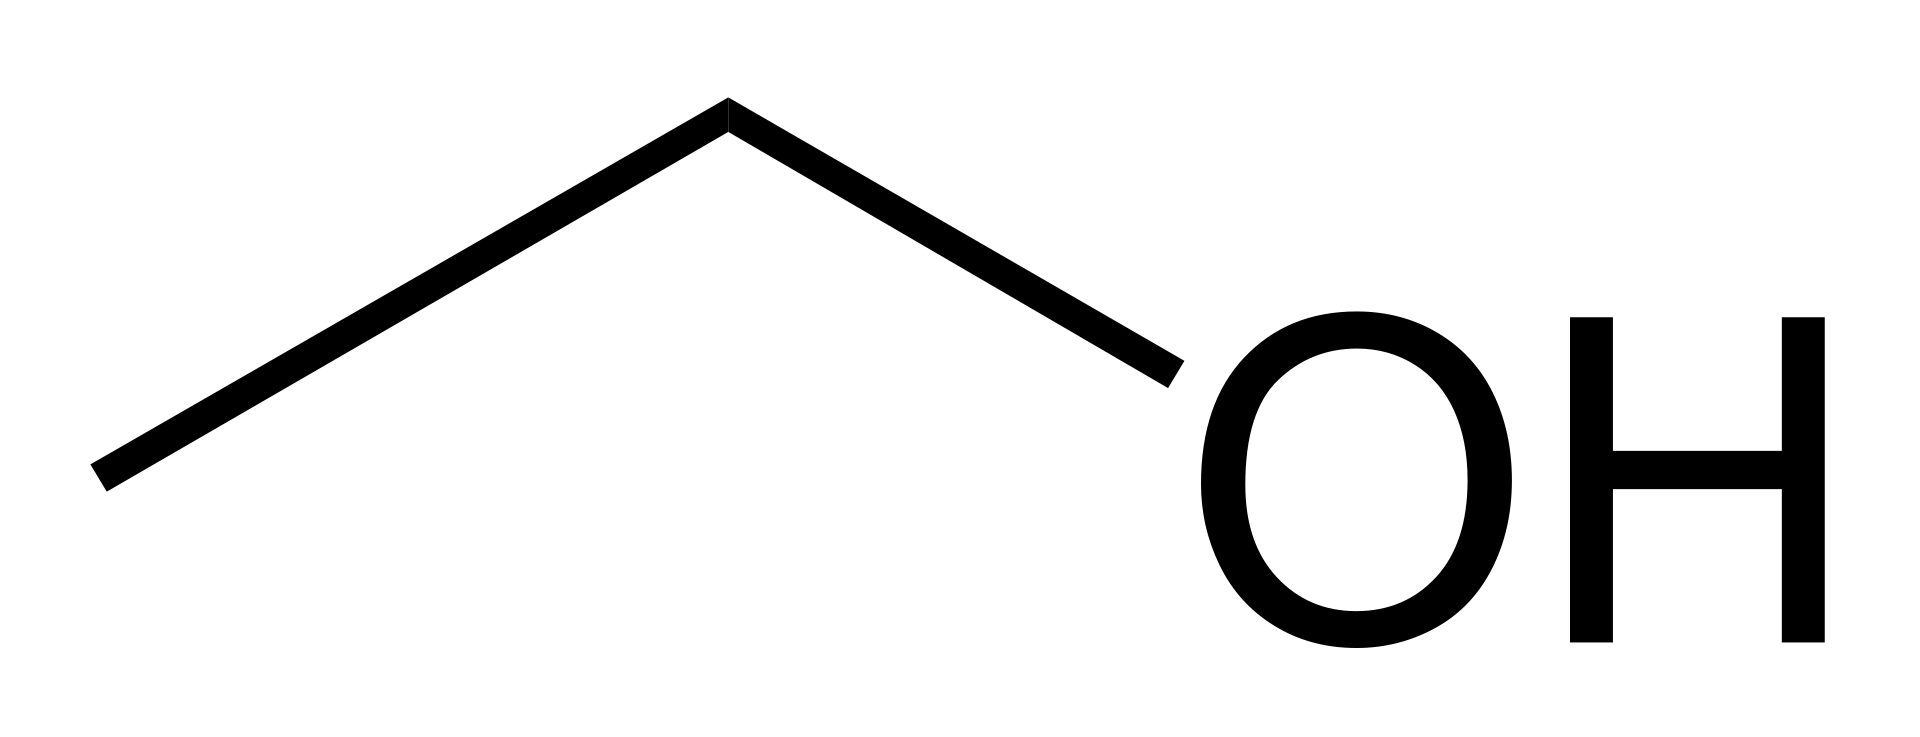
\includegraphics[width=\linewidth]{ethanol.png}
        \caption{Ethanol}
      \end{subfigure}
    \caption{ Molecular Structures of Sample Alcohol Types}
    \label{fig:mol}
\end{figure}
As we can see, there are not many significant differences and are a lot of 
similarities across the molecular structures of all the selected alcohols. 
Thus, to distinguish different alcohols, the following features (in a 
molecular structure) will be used:\\
- Number of oxygen atoms\\
- Number of carbon atoms\\
- Number of single bonds, which also represents the number of hydrogen atoms\\
- The length of the main carbon chain\\
- The position(s) of the hydroxyl group(s)\\
To differentiate between different mixtures, the following features will be used:\\
- Number of water molecules\\
- Number of alcohol molecules\\
We can also see that glycerol is the only alcohol type that possess 3 hydroxyl 
groups while propylene glycol is really close to 1,3-propanediol 
(only different in the position of the 2nd hydroxyl group). Meanwhile, 
ethanol is quite similar to methanol and 1-propanol is a structural isomer 
of 2-propanol. Interestingly, among all the above alcohol types, methanol 
is the only type that is less viscous than water.

\section{Machine Learning Implementation}
Two sets of data will be prepared: a training data set and a testing data set. 
The training data set is used to construct the model while the testing data 
set is left unused throughout the training process and only used in 
approximating the true error so that the model is not overfit. We will make 
a model of thermal conductivity and a model of viscosity.

The parameter set for each model are decided by using k-fold methods. 
Within the possible range of parameters, every combination of parameters 
is cross-validated using the k-fold methodology and then the training 
performance scores are compared. The parameter set of the model that has 
the best training performance score will be chosen.
The selected parameter sets will be used to create the models with the 
training data set. The constructed models will then be tested on the 
testing data set to obtain the performance score. 

To thoroughly analyze the machine learning implementation, the training 
data set and testing data set will be decided by 2 ways: 
random and out of sample.
The random method is to randomly divided the entire data set into the 
training data set and the testing data set and create the models. 
The resulting models will be used to progress to the final step.
The out of sample method is to completely exclude an alcohol type out of 
the training sample. Four alcohol types, namely propylene glycol, methanol. 
2-propanol and glycerol, will be in turn excluded to assess the 
characteristics of machine learning approach in this problem.

The performance score of the testing and training processes will be 
calculated using the $R^2$ score method as follows:
\begin{equation}
    R^{2}=1-\frac{S S R}{T S S}
\end{equation}
Where
\begin{equation}
    S S R=\sum_{i=1}^{n}\left(y_{i}-f\left(x_{i}\right)\right)^{2}
\end{equation}
\begin{equation}
    T S S=\sum_{i=1}^{n}\left(y_{i}-\frac{1}{n} \sum_{j=1}^{n} y_{j}\right)^{2}
\end{equation}
Furthermore, SSR stands for squared sum of residual, TSS stands for total squared sum, 
y is the real value, $f(x_i)$ is the predicted value, n is the number of data in 
the data sample and i and j are data indices.
\section{Optimization}
In the optimization step, I will find the optimal values of desired properties 
while returning the corresponding inputs, which is the structural features in 
this work. The finding is done by setting up an optimization problem with an 
objective function and different constraints. The objective function guides 
the computer to find the optimal results while the constraints help us to 
remove the unrealistic outcomes.\\
This work considers optimization of thermal conductivity and viscosity. 
Thus, the problem will be described as follows:\\
Maximize:
\begin{equation}
    \alpha \frac{T C-\overline{T C}}{\sigma_{T C}}-\beta \frac{V i s c-\overline{V i s c}}{\sigma_{V i s c}}
    \label{eq:obj} 
\end{equation}
Subject to:\\
- The number of alcohol molecules $>$ 0\\
- The number of carbons and oxygens $>$ 0\\
- The position of OH groups $>$ 0\\
- The length of the main carbon chain $<$ the number of carbons\\
- The number of total molecules $<$ 2100 (estimated number that fits in the investigated volume)\\
- Every input is integer\\
Where $\alpha$ and $\beta$ are the weighting factors that define the importance of the 
thermal conductivity and viscosity. In this research, we value the thermal 
conductivity and the viscosity equally, which means $\alpha=\beta=1$. $\sigma_{T C}$ is the standard 
deviation of the sample thermal conductivity values, $\sigma_{Visc}$ is the standard 
deviation of the sample viscosity values, $\overline{T C}$ is the mean of the sample 
thermal conductivity values and $\overline{V i s c}$ is the mean of the sample viscosity 
values. The values of thermal conductivity and viscosity will be first 
standardized before processed in the objective function \ref{eq:obj}.



 %Input chap3.tex
\chapter{Results and Discussions} %Chapter 4 Title
% Need a chapter for results and results discussion
\section{Simulation Results}
The calculated properties from Molecular Dynamics simulations are presented 
in the following forms
\begin{figure}[h!]
    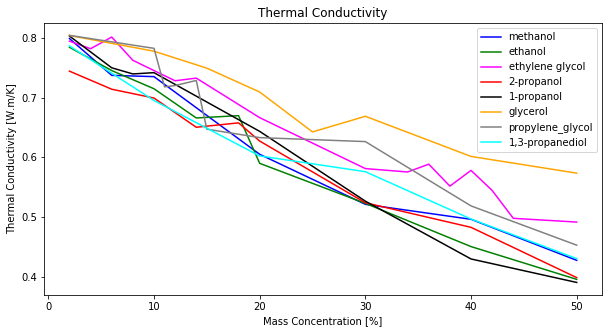
\includegraphics[width=1\textwidth]{tc.png}
    \centering
    \captionsetup{justification=centering}
    \caption{Thermal Conductivity Values of 8 Sample Alcohol Types Across Mass Concentration}
\end{figure}

As expected in the thermal conductivity graph, all the thermal conductivity 
lines decreased due to the fact that all types of alcohol are less efficient 
than water in terms of heat transfer. Even though having a decreasing trend, 
the gradient of the thermal conductivity line of glycerol was quite different 
compared to others. Due to the absence of enthalpy quantity, all values 
converge to approximately 0.85 [W/m.K], which is expected.
\begin{figure}[h]
    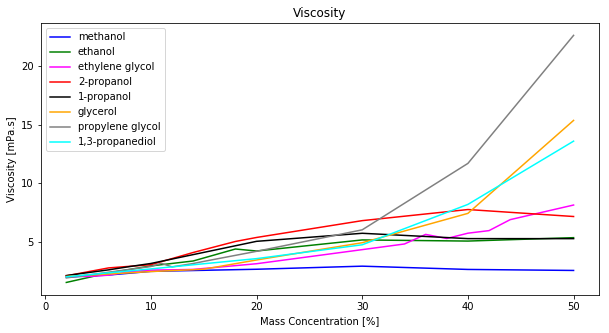
\includegraphics[width=1\textwidth]{visc.png}
    \centering
    \captionsetup{justification=centering}
    \caption{Viscosity Values of 8 Sample Alcohol Types Across Mass Concentration}
\end{figure}

In the viscosity graph, while all values converged to the value of pure water, 
which is expected, the viscosity line of methanol also decreased as methanol 
is less viscous than water.
\section{Model Result Analysis}
As mentioned in the method section, the training data will be defined in 5 
different ways: randomly divided, excluding all propylene glycol data, 
excluding all glycerol data, excluding all methanol data and excluding all 
2-propanol data. The result for each data division approach is presented as 
follows:
\begin{table}[ht]
    \centering
    \caption{Performance Score on the Testing Data Set}
    \begin{tabular}{|c|c|c|}
        \hline
        \hline
        Training Data & TC $R^2$ Score & Visc $R^2$ Score\\
        \hline
        Randomly divided & 0.96  & 0.70\\
        Propylene Glycol data excluded & 0.86  & 0.74\\
        Glycerol data excluded & 0.36  & 0.76\\
        Methanol data excluded & 0.92 & Failed\\
        2-propanol data excluded & 0.90  & 0.72\\
        \hline
    \end{tabular}
    \label{table:1}
\end{table}

The results indicate that for any alcohol that has structural similarities 
with data in the training set, has a high performance score when used on 
the testing data set. However, the alcohols that are significantly different 
from the training sets have a quite low performance scores.

For thermal conductivity models, except for glycerol-excluded approach model, 
all the models possess a decent performance score. The explanation for this is 
that the testing sets in such cases are similar to the training sets. While 
propylene glycol - 1,3-propanediol and 1-propanol - 2-propanol are pairs of 
structural isomers, methanol is also quite close to ethanol. However, even 
though the molecular structure of glycerol is not so distinguished to the 
others, it is the only type of alcohol that had the gradient of the thermal 
conductivity that trends significantly different from the others; not to 
mention that glycerol is the only type of alcohol that possesses 3 hydroxyl 
groups within the molecule. This helps to explain why the glycerol-excluded 
model performance score is quite low.

A similar explanation can be applied to explain the phenomenon in the 
viscosity models. In methanol-excluded model, the model failed to predict 
the viscosity values of methanol. Recalling the simulation data in the 
previous sub-section, methanol was the only type of alcohol that had a 
non-increasing value trend. It came from the fact that within the sample, 
methanol is the only type of alcohol that is less viscous than water. In 
other words, methanol is very different from the other alcohols when looking 
from a viscosity point of view. Thus, the model could not predict the 
viscosity values of methanol since it did not learn any methanol similar 
relationship during the training process. The other models have moderate 
performance scores but are not satisfactory. Since these models included 
methanol in the training process, it is likely that the bizarre viscosity 
of methanol influenced the prediction ability and resulted in non-satisfactory 
performance scores.

For future improvement of this method, the sample alcohol types should be 
diversified to obtain more generalized prediction models. Since low viscosity 
of methanol is a good point, we should include more alcohol types that are 
less viscous than water. However, there might be a chance that the selected 
variables are not sufficient to cover abnormal cases. Thus, independent 
research on how molecular structures influence the thermophysical properties 
of unusual alcohol types like methanol should be conducted to improve the 
variable sets. At the same time, we also need to diversify the sample in terms 
of structural features. Obviously, the sample alcohol types only have single 
bonds and straight carbon chain. Thus, the addition of double bonds, triple 
bonds, circle structures and tree-like carbon chain could help generalize the 
solutions.

While including methanol in the construction of models can give us a better 
direction to prepare data and investigate on a certain direction, I will 
exclude methanol out of the construction of the model in order to investigate 
the capability of this methodology for prediction when performance scores are 
sufficiently high. The expected performance score should be significantly 
higher than the previous version. Thus, the finalized models performance 
scores become
\begin{table}[ht]
    \centering
    \caption{Finalized Models Performance Scores}
    \begin{tabular}{|c|c|}
        \hline
        \hline
        Thermal Conductivity $R^2$ Score & Viscosity $R^2$ Score\\
        \hline
        0.96  & 0.91\\
        \hline
    \end{tabular}
    \label{table:2}
\end{table}

The models also help us to investigate how variables influence the 
thermophysical properties using the F-score method \cite{sasaki_truth_2007}. 
For the final models, the variable influences (feature importance) 
are as follows:

\begin{figure}[ht]
    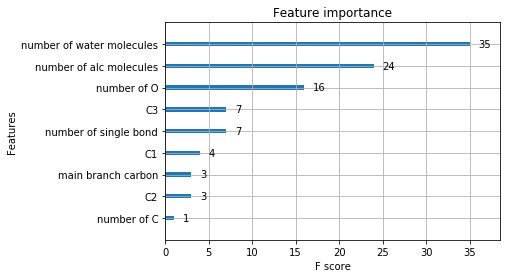
\includegraphics[width=1\textwidth]{fitc.png}
    \centering
    \captionsetup{justification=centering}
    \caption{Feature Importance of the Thermal Conductivity Model}
\end{figure}
\begin{figure}[ht]
    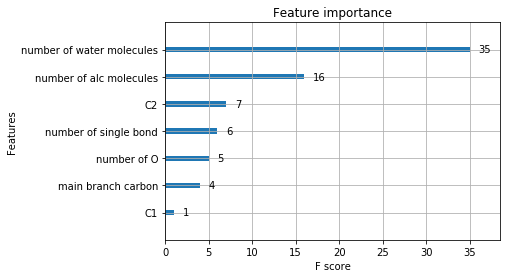
\includegraphics[width=1\textwidth]{fiv.png}
    \centering
    \captionsetup{justification=centering}
    \caption{Feature Importance of the Viscosity Model}
\end{figure}
\newpage

As expected, the mass concentration is one of the main factors that decides 
the thermal properties of the mixtures by having the number of water molecules 
and alcohol molecules as the highest influential variables. However, due to 
some noises and possibly the lack of better variables in the viscosity model, 
the score of the number of alcohol molecules is slightly underestimated or the 
score of the number of water molecules is slightly overestimated. Nonetheless 
the importance of these 2 variables are still clearly shown.\\
For thermal conductivity, another research \cite{manjunatha_investigation_2017} also showed that 
the number of hydroxyl groups affect the heat transfer ability of the alcohol. 
Interestingly, by using machine learning approach, we can also know that the 
hydroxyl group at the 3rd carbon position in the main carbon chain and the 
number of single bonds also have a significant influence on the thermal 
conductivity.\\
For viscosity, it is the hydroxyl group at the 2nd carbon position in the 
main carbon chain that significantly affect the viscosity values.

\section{Optimization Results}
Using the formulation \ref{eq:obj} and the related constraints, the results for 
optimization showed that the alcohol types with the following estimated 
structural features will have the optimal performance on both thermal 
conductivity and viscosity:
\begin{table}[ht]
    \centering
    \caption{Predicted Structural Features From Optimization}
    \begin{tabular}{|c|c|c|c|c|c|c|c|}
        \hline
        \hline
        \thead{Ratio of Molecules \\ (alcohol/water)} & \thead{Number of \\carbon} & \thead{Number of \\oxygen}
        & \thead{Number of \\single bond} & \thead{Length of \\(main) \\ (carbon chain)} & \thead{Position of \\hydroxyl \\groups}\\
        \hline
        0.0005-0.0148  & 3-4 & 3 & 13,17 & 3 & 1, 2, 3\\
        \hline
    \end{tabular}
    \label{table:opt}
\end{table}
\begin{table}[ht]
    \centering
    \caption{Predicted Thermophysical Properties From Optimization}
    \begin{tabular}{|c|c|}
        \hline
        \hline
        \thead{Predicted Thermal Conductivity\\ (W/m.K)}& \thead{Predicted Viscosity \\(mPa.s)}\\
        \hline
         0.81219405 & 2.0989997\\
        \hline
    \end{tabular}
    \label{table:prop}
\end{table}

As we can see, the best mixture is almost water, as water so far has the best 
thermal conductivity and viscosity. Furthermore, one of the molecular 
structures that can be constructed from these predicted features is glycerol, 
which is the type of alcohol that has the highest thermal conductivity and 
quite good viscosity across mass concentrations of alcohol-water mixtures 
according to the simulated data. This is showing that the methodology is 
approaching on the right direction. In the future work, with the additional 
constraint of freezing point, the method will be able to produce the desired 
outcome. Even though we obtained the features, the lack of diversity in terms 
of molecular structure from the sample data prevents us from constructing a 
complete structure. Thus, in the future where this method is applied, the 
sample data need to be sufficiently diverse enough as discussed in the 
previous sub-section. At the same time, an interpreting method should also be 
developed to translate from the broken down molecular structural features to 
a complete structure. %Input chap4.tex
\chapter{Conclusion} %Chapter 5 Title
The introduction section showed that there are several obstacles that 
prevent us from getting a research direction towards the next generation 
of antifreeze. In this study, I suggested that such problems can be overcome 
by creating a function that connects the antifreeze structural features to 
its thermophysical properties such as thermal conductivity and viscosity. 
The function is created by implementing a supervised machine learning method 
called xgboost while the data used in training xgboost models is obtained 
from Green-Kubo relation based molecular dynamics simulations of 8 types of 
alcohol: methanol, ethanol, ethylene glycol, glycerol, 1-propanol, 2-propanol, 
1,3-propanediol and propylene glycol. Such a function helps us to gain clues 
for constructing the next generation of alcohol coolants while it also shows 
us a research direction to optimize this method in the future.
\section*{Summary of Findings}
The training data is decided by 5 different ways: randomly divided, 
excluding methanol, excluding 2-propanol, excluding glycerol and excluding 
propylene glycol. The results showed that the models can predict values that 
have similar patterns to training data, while they had difficulty predicting 
properties that were very different to the training data. Thus, to overcome 
this problem in the future, there are 2 different approaches: diversification 
of the training data and conducting of research on special alcohol types such 
as methanol.\\
The machine learning approach can also statistically show that besides factors 
such as the concentration and number of hydroxyl groups, the hydroxyl group at 
the 3rd carbon position in the main carbon chain can significantly affect the 
thermal conductivity values. Similarly, the hydroxyl group at the 2nd carbon 
position in the main carbon chain has a significant influence on the viscosity 
values.\\
For the given alcohol sample excluding methanol, the optimization predicted 
that the next alcohol antifreeze candidate would possess 3 to 4 carbons, 3 
oxygens, 13 or 17 single bonds, a main carbon chain of length 3 and have 
hydroxyl groups in every position. However, the concentration showed that 
the mixture is almost water, which makes sense since we are only considering 
the thermal conductivity and viscosity. Furthermore, one of molecular 
structures that can be constructed from the predicted structural features is 
glycerol, the type of alcohol that has the highest thermal conductivity and 
fairly low viscosity across mass concentration of alcohol-water mixtures 
according to simulated data. Thus, the results show that the optimization 
algorithm approaches the problem in an appropriate manner. With the addition 
of freezing point in the future, the methodology will be able to produce 
desired outputs. 
Furthermore, the prediction is likely to be further improved with a more 
diverse sample data. An interpreting method is also needed to translate the 
obtained structural feature values to a complete final structure.
 %Input chap5.tex

%\appendix
%\addcontentsline{toc}{chapter}{Appendices}
%\chapter*{Appendix A: Data Table}
%\begin{table}[h!]
    \begin{center}
      \caption{Autogenerated table from .csv file.}
      \label{table1}
      \pgfplotstabletypeset[
        multicolumn names, % allows to have multicolumn names
        col sep=comma, % the seperator in our .csv file
        display columns/0/.style={
          column name=$Value 1$, % name of first column
          column type={S},string type},  % use siunitx for formatting
        display columns/1/.style={
          column name=$Value 2$,
          column type={S},string type},
        every head row/.style={
          before row={\toprule}, % have a rule at top
          after row={
              \si{\ampere} & \si{\volt}\\ % the units seperated by &
              \midrule} % rule under units
              },
          every last row/.style={after row=\bottomrule}, % rule at bottom
      ]{thesisdata.csv} % filename/path to file
    \end{center}
  \end{table}
\bibliographystyle{apacite}
\bibliography{mybib}
\end{document}